%%%%%%%%%%%%%%%%%%%%%%%%%%%%%%%%%%%%%%%%%%%%%%%%%%%%%%%%%%%%%%%%%%%%%%%%%%%
%%
%% Copyright (c) 2014 Adobe Systems Incorporated. All rights reserved.
%%
%% Licensed under the Apache License, Version 2.0 (the "License");
%% you may not use this file except in compliance with the License.
%% You may obtain a copy of the License at
%%
%% http://www.apache.org/licenses/LICENSE-2.0
%%
%% Unless required by applicable law or agreed to in writing, software
%% distributed under the License is distributed on an "AS IS" BASIS,
%% WITHOUT WARRANTIES OR CONDITIONS OF ANY KIND, either express or implied.
%% See the License for the specific language governing permissions and
%% limitations under the License.
%%
%%%%%%%%%%%%%%%%%%%%%%%%%%%%%%%%%%%%%%%%%%%%%%%%%%%%%%%%%%%%%%%%%%%%%%%%%%%
\documentclass{beamer}
% Theme Matrix: http://www.hartwork.org/beamer-theme-matrix/
\mode<presentation> { \usetheme{Malmoe}\usecolortheme{dove} }
\setbeamertemplate{itemize items}[default]
\usepackage[T1]{fontenc}
\usepackage{parskip,graphics,tikz,multimedia,hyperref,ulem,multicol}
\usetikzlibrary{arrows,positioning,shapes,decorations.pathmorphing,
  decorations.markings}
\setlength{\itemsep}{0pt}\setlength{\parskip}{0pt}\setlength{\parsep}{0pt}
\graphicspath{{./images/}}

\usepackage{listings,textcomp,color}
\lstset{language=Python,upquote=true,
  basicstyle=\ttfamily\tiny,numbers=left,
  numberstyle=\tiny,stepnumber=1,numbersep=5pt,
  backgroundcolor=\color{white},frame=single,tabsize=2,
  showspaces=false,showstringspaces=false,showtabs=false,
  breaklines=true,breakatwhitespace=true,escapeinside=||,
  keywordstyle=\color{blue!70},stringstyle=\color{green!70!black!70},
  commentstyle=\color{black!80}\it
}
\lstdefinelanguage{scala}{
  morekeywords={abstract,case,catch,class,def,%
    do,else,extends,false,final,finally,%
    for,if,implicit,import,match,mixin,%
    new,null,object,override,package,%
    private,protected,requires,return,sealed,%
    super,this,throw,trait,true,try,%
    type,val,var,while,with,yield},
  otherkeywords={=>,<-,<\%,<:,>:,\#,@},
  sensitive=true,
  morecomment=[l]{//},
  morecomment=[n]{/*}{*/},
  morestring=[b]",
  morestring=[b]',
  morestring=[b]"""
}

\usebackgroundtemplate{
  \tikz[overlay,remember picture]
  \node[yshift=10mm,anchor=south east,inner sep=0pt]
    at (current page.south east) {
    \includegraphics[width=0.5in]{logo}
  };
}

\tikzset{
  yn/.style={draw,thick,rounded corners,fill=yellow!20,inner sep=.3cm},
  bn/.style={draw,thick,rounded corners,fill=blue!05,inner sep=.3cm},
  on/.style={draw,thick,rounded corners,fill=orange!20,inner sep=.3cm},
  rn/.style={draw,thick,rounded corners,fill=red!20,inner sep=.3cm},
  wn/.style={draw,thick,rounded corners,inner sep=.3cm},
  greenn/.style={draw,thick,rounded corners,fill=green!20,inner sep=.3cm},
  grayn/.style={draw,thick,rounded corners,fill=gray!20,inner sep=.3cm},
  to/.style={
    ->,>=stealth',shorten >=1pt,semithick,font=\sffamily\footnotesize
  },
  from/.style={
    <-,>=stealth',shorten >=1pt,semithick,font=\sffamily\footnotesize
  },
  tofrom/.style={
    <->,>=stealth',shorten >=1pt,semithick,font=\sffamily\footnotesize
  },
  every node/.style={align=center},
  squig/.style={->,line join=round,decorate, decoration={zigzag,
    segment length=8,amplitude=2,post=lineto,post length=2pt}}
}

\expandafter\def\expandafter\insertshorttitle\expandafter{%
  \insertshorttitle\hfill%
  \insertframenumber\,/\,\inserttotalframenumber}
\renewcommand*{\thefootnote}{\fnsymbol{footnote}}
\beamertemplatenavigationsymbolsempty

\begin{document}

\title[Spindle, CloudCom 2014]{
  {\Large Performance study of Spindle, a web analytics\\[-2mm]
    query engine implemented in Spark} \\[-3mm]
  {\small CloudCom 2014}
}
\author[Amos and Tompkins, Adobe Research]{
  {\bf Brandon Amos$^*$} and David Tompkins, {\bf Adobe Research } \\
  {\footnotesize
    $^*$Adobe summer intern, Ph.D. Student at
    Carnegie Mellon University.} \\[4mm]
  \vspace*{-5mm}
}
\date{December 19, 2014}
{\setbeamertemplate{footline}{}\setbeamertemplate{headline}{}\frame{\titlepage}}
\addtocounter{framenumber}{-1}

\section{Motivation}
\frame{\frametitle{\insertsection}
  \begin{itemize}
    \item Adobe Marketing Cloud offers web analytics.
  \end{itemize}
  \pause
  \begin{center}
    \begin{tikzpicture}[every node/.style={anchor=north}]
      \node at (0,0) {\includegraphics[width=1\textwidth]{tpbb1.png}};
      \pause
      \node at (0,0) {\includegraphics[width=1\textwidth]{tpbb2.png}};
    \end{tikzpicture}
  \end{center}
}

\frame{\frametitle{\insertsection}
  \begin{itemize}
    \item Adobe Marketing Cloud offers web analytics.
    \item<+-> Terabytes of data, thousands of servers.
    \item<+-> Trending general-purpose distributed data processing engines.
      \begin{itemize}
      \item<+-> Apache Spark
        \begin{itemize}
        \item<+-> Queries implemented with map and reduce functions.
        \item<+-> In-memory caching.
        \end{itemize}
      \item<+-> Cloudera Impala
      \item<+-> Google Dremel
      \end{itemize}
    \item<+-> We present {\bf Spindle}, which is an early investigation of the
      feasibility of Apache Spark for web analytics
    \item<+-> {\bf Problem:} How well does Spindle scale for
      web analytics?
  \end{itemize}
}

\section{Spindle Architecture}

\subsection{Overview.}
\frame{\frametitle{\insertsection}\framesubtitle{\insertsubsection}
  What is Spindle?
  \pause
  \begin{center}
  \scalebox{0.65}{
  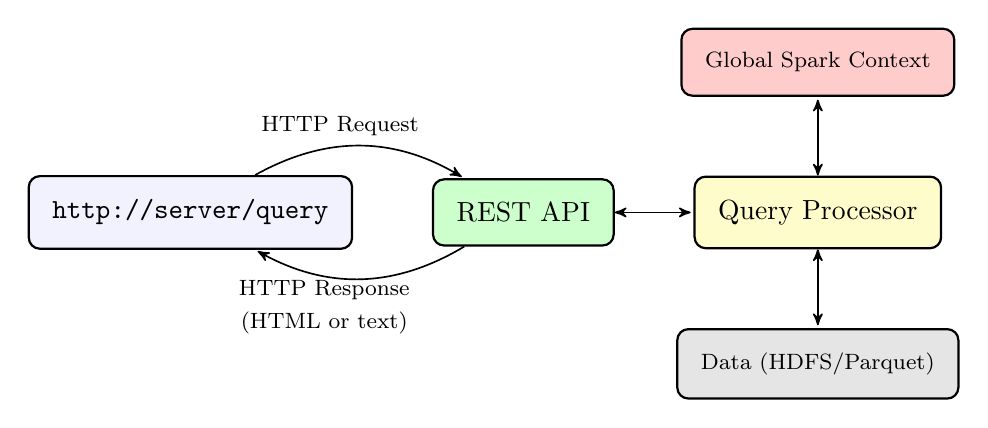
\begin{tikzpicture}
    \node[bn] (query) {{\tt http://server/query}};
    \pause

    %% \node[left=of query,align=left] () {{\bf Parameters:}\\ Date Range\\Spark Tuning Options};
    %% \pause

    \node[greenn,right=of query] (spray) {REST API};
    \node at (1.9cm,1.1cm) {{\footnotesize HTTP Request}};
    \node at (1.7cm,-1.2cm)
      {{\footnotesize HTTP Response}\\{\footnotesize (HTML or text)}};
    \draw[to] (query) edge [bend left] (spray);
    \draw[to] (spray) edge [bend left] (query);
    \pause

    \node[yn,right=of spray] (queryservice) {Query Processor};
    \draw[tofrom] (spray) -- (queryservice);
    \pause

    \node[rn,above=of queryservice] (sc)
      {{\footnotesize Global Spark Context}};
    \draw[tofrom] (queryservice) -- (sc);
    \pause

    \node[grayn,below=of queryservice] (db)
      {{\footnotesize Data (HDFS/Parquet)}};
    \draw[tofrom] (queryservice) -- (db);
  \end{tikzpicture}
  }
  \end{center}
}

\frame{\frametitle{\insertsection}\framesubtitle{\insertsubsection}
  \begin{itemize}
  \item<+-> Operates on archival data with 250 columns.
  \item<+-> Data is sparse and queries use <10 columns at a time.
  \item<+-> Use columnar data format on distributed filesystem.
  \item<+-> Parameters when processing data.
    \begin{itemize}
    \item<+-> Intermediate data partitioning
    \item<+-> Caching
    \end{itemize}
  \end{itemize}
}


\subsection{Queries.}
\newcommand{\nameMapsRow}[2]{#2 & #1 \\}
\newcommand{\mt}{\ensuremath{\times}}
\frame{
\begin{table}[hb]
  \centering
  \scriptsize
  \begin{tabular}{rl}
    Shorthand & Name \\ \hline
    \nameMapsRow{Pageviews}{Q0}
    \nameMapsRow{Revenue}{Q1}
    \nameMapsRow{RevenueFromTopReferringDomains}{Q2}
    \nameMapsRow{RevenueFromTopReferringDomainsFirstVisitGoogle}{Q3}
    \nameMapsRow{TopPages}{Q4}
    \nameMapsRow{TopPagesByBrowser}{Q5}
    \nameMapsRow{TopPagesByPreviousTopPages}{Q6}
    \nameMapsRow{TopReferringDomains}{Q7}
  \end{tabular}
\end{table}
\bigskip
\pause
\begin{table}[ht]
  \centering
  \scriptsize
  \begin{tabular}{ccccccccc}
  &
    Q0 &  Q1  &  Q2  &  Q3  &  Q4  &  Q5  &  Q6  &  Q7  \\ \hline
  post\_pagename &
   \mt &      &      &      &  \mt &  \mt &  \mt &      \\
  user\_agent &
       &      &      &      &      &  \mt &      &      \\
  visit\_referrer &
       &      &  \mt &  \mt &      &      &      &      \\
  post\_visid\_high &
       &      &  \mt &  \mt &      &      &  \mt &  \mt \\
  post\_visid\_low &
       &      &  \mt &  \mt &      &      &  \mt &  \mt \\
  visit\_num &
       &      &  \mt &  \mt &      &      &  \mt &  \mt \\
  visit\_referrer &
       &      &      &      &      &      &      &  \mt \\
  hit\_time\_gmt &
       &      &      &      &      &      &  \mt &      \\
  post\_purchaseid &
       &  \mt &  \mt &  \mt &      &      &      &      \\
  post\_product\_list &
       &  \mt &  \mt &  \mt &      &      &      &      \\
  first\_hit\_referrer &
       &      &      &  \mt &      &      &      &      \\
  \end{tabular}
\end{table}
}

\section{Empirical Results} %TODO: Add summaries.
\subsection{Caching.}
\frame{\frametitle{\insertsection}\framesubtitle{\insertsubsection}
  \begin{itemize}
    \item<+-> Six cluster nodes (32 GB memory each), Spark and HDFS on each.
    \item<+-> 13.1GB of data, 1 week, 1 customer.
    \item<+-> {\bf Question:} How does caching in-memory improve performance?
  \end{itemize}
}

\frame{
  \centering
  \begin{tikzpicture}[every node/.style={anchor=south west}]
    \node at (0,0)(){\includegraphics[width=1\textwidth]{results-2014.08.02/caching/caching.pdf}};
    \fill[white] (1.4,0.95) rectangle (11,6) {};
    \fill[white] (6,6) rectangle (9,7) {};
    \pause
    \node at (0,0)(){\includegraphics[width=1\textwidth]{results-2014.08.02/caching/caching.pdf}};
    \fill[white] (3.5,0.95) rectangle (5.5,6) {};
    \fill[white] (6.5,0.95) rectangle (8.6,6) {};
    \fill[white] (6,6) rectangle (9,7) {};
    \pause
    \node at (0,0)(){\includegraphics[width=1\textwidth]{results-2014.08.02/caching/caching.pdf}};
    \fill[white] (7.5,0.95) rectangle (8.6,7) {};
    \pause
    \node at (0,0)(){\includegraphics[width=1\textwidth]{results-2014.08.02/caching/caching.pdf}};
  \end{tikzpicture}
}

\subsection{Benchmarking concurrent queries.}
\frame{\frametitle{\insertsection}\framesubtitle{\insertsubsection}
  \begin{itemize}
    %\item<+-> Multiple users can utilize an analytics system like SiteCatalyst
    %  concurrently, and Spark can be used in multithreaded applications.
    \item<+-> How much will Spindle's performance
      degrade if multiple users are utilizing it at the same time?
    \item<+-> Concurrently call the same query on the same data.
    \item<+-> Average execution times.
    %\item<+-> {\bf Solution:} Assume users submit the same query
    %  at the same time and observe the average query response time.
    %% \item<+-> A Python script using threading manages threads for
    %%   each number of concurrent queries.
    %% \item<+-> Consider the example below for 2 threads and 3 repeated
    %%   queries per thread. The first thread finishes before the second,
    %%   and remains loaded until the second thread finishes.
    %%   $t_4^1$ and $t_5^1$ are not used in the average.
    %% \item<+-> This experiment runs queries on the date range of
    %%   Jan 1, 2014 to Jan 7, 2014 and each thread calls the query 4 times.
  \end{itemize}
}

\newcommand{\revealConcurrent}[1]{
  \frame{
    \begin{tikzpicture}[every node/.style={anchor=south west}]
      \node at (0,0)(){\includegraphics[width=\textwidth]{#1}};
      \fill[white] (1.5,0.95) rectangle (10,6.8) {};
      \pause
      \node at (0,0)(){\includegraphics[width=\textwidth]{#1}};
    \end{tikzpicture}
  }
}
\revealConcurrent{results-2014.08.02/concurrent/pdf/TopPages.pdf}
\revealConcurrent{results-2014.08.02/concurrent/pdf/TopPagesByPreviousTopPages.pdf}

\subsection{Scaling Spark and HDFS workers.}
\frame{
  \centering
  \begin{tikzpicture}[every node/.style={anchor=south west}]
    \node at (0,0)(){\includegraphics[width=1\textwidth]{images/scalingWorkers.pdf}};
    \fill[white] (2,0.95) rectangle (8,6.5) {};
    \pause
    \node at (0,0)(){\includegraphics[width=1\textwidth]{images/scalingWorkers.pdf}};
  \end{tikzpicture}
}


\section{Conclusions}
\frame{\frametitle{\insertsection}\framesubtitle{\insertsubsection}
  \begin{itemize}
    %\item<+-> Spark is a good candidate for expressing web analytics queries.
  \item<+-> We present {\bf Spindle}, which is an open-source prototype analytics processing
    engine.
      \begin{itemize}
      \item<+-> Sample set of web analytics queries.
      \item<+-> REST-based interface to tune parameters.
      \end{itemize}
    \item<+-> Spindle's future work is on preprocessing.
  \end{itemize}
  \pause
  \vspace{4mm}
  \begin{center}
    {\scriptsize
      \begin{tabular}{r|l}
      Spindle Project & \url{http://github.com/adobe-research/spindle} \\
      Demo & \url{http://adobe-research.github.io/spindle/} \\
      Brandon Amos & \url{http://github.com/bamos} \\
      David Tompkins & \url{http://github.com/DavidTompkins} \\
      \end{tabular}
    }
  \end{center}
}

\end{document}
